\chapter{Design and Implementation}\label{chap:design-implementation}

\section{System Architecture Overview (PC--Android System Design)}\label{sec:4-1}
The system is designed in a client--server architecture with a central PC controller coordinating multiple Android capture devices (see ADR-001: Reactive State Management for the rationale behind this architectural choice). The PC application serves as the master controller, discovering and connecting to each Android device over a local network. Each Android device runs a capture app responsible for recording sensor data and video, while the PC provides a unified interface to start/stop recordings and aggregate data.

The system architecture (see Figure~\ref{fig:4_01_arch_overview} in Appendix I) demonstrates how the PC communicates with each Android smartphone via Wi-Fi using a custom TCP/IP protocol, sending control commands and receiving live telemetry (video previews, sensor readings). The Android devices operate largely autonomously during capture -- each uses its own high-precision clock to timestamp data locally -- but all devices are synchronised to the PC's timeline through network time alignment. This design allows multiple phones to record simultaneously under one session, with the PC as the authoritative time base. The PC can also integrate local hardware (e.g., a webcam and GSR sensor connected directly) alongside the Android data. All captured modalities (video streams, audio, thermal data, GSR signals) are temporally aligned and later consolidated on the PC. The result is a distributed recording system in which heterogeneous data sources behave like a single synchronised apparatus.

\section{Android Application Design and Sensor Integration}\label{sec:4-2}
On the Android side, the application is structured to handle multi-modal data capture in a coordinated fashion. At its core is a \texttt{RecordingController} class that manages all hardware components and recording tasks. This controller prepares each subsystem -- cameras (RGB and thermal), physiological sensors (GSR/PPG), microphone, etc. -- and triggers them in sync. When a recording session starts, the controller initializes a new session directory and then concurrently starts each enabled sensor/camera capture with nanosecond-precision timestamps. Each modality's data is written to device storage in real time. The design relies on Android's modern libraries for robust performance: CameraX is used for efficient video and image capture [13], and the Nordic BLE library for reliable Bluetooth Low Energy communication with sensors [14]. Crucially, all sensor readings and frames are timestamped using a monotonic clock source to ensure internal consistency. The app architecture cleanly separates concerns -- for example, camera handling is in an \texttt{RgbCameraManager}, thermal imaging in a \texttt{TopdonThermalCamera} module, and GSR sensing in a \texttt{ShimmerGsrSensor} class -- each exposing a common interface for the controller to start/stop streams. This modular design (following principles outlined in ADR-003: Function Decomposition Strategy) makes it easy to enable or disable features based on device capabilities (e.g., if a phone has no thermal camera attached, that module remains inactive). It also simplifies synchronisation logic, since the controller can treat each data source uniformly (start all, stop all) and trust each to timestamp its output.

The Android app's internal architecture for thermal camera integration is detailed in Figure~4.2 (see Appendix I), which provides an overview of the data flow and component interactions.

The following subsections detail the integration of the Topdon thermal camera and Shimmer GSR sensor in the Android app.

\subsection{Thermal Camera Integration (Topdon)}\label{sec:4-2-1}
Integrating the Topdon TC001 thermal camera on Android required using USB host mode and a UVC (USB Video Class) library. The app utilises the open-source Serenegiant USB Camera library (UVCCamera) for USB Video Class device support [16] to interface with the device. A dedicated class \texttt{TopdonThermalCamera} implements the \texttt{ThermalCamera} interface and encapsulates all thermal camera functionality. When the camera is physically connected via USB-C, an Android USB monitor detects the device. The \texttt{TopdonThermalCamera} registers a \texttt{USBMonitor.OnDeviceConnectListener} to handle attachment events. On a successful connection, it opens the UVC device and configures it to the desired frame size and mode before starting the video stream [16]. By default, the camera is set to its native thermal resolution (256\,\texttimes\,192 pixels) and begins previewing immediately on a background thread.

For each incoming thermal frame, the library provides a framebuffer in \texttt{ByteBuffer} format. The implementation registers a frame callback to retrieve this data stream. In the callback, the code reads the raw temperature data from the buffer as an array of 16-bit (or 32-bit) values and writes each frame's timestamp and temperature data to a CSV file: each row corresponds to one frame, beginning with a high-resolution timestamp (in nanoseconds), followed by the temperature values of all 49{,}152 pixels (256\,\texttimes\,192) in that frame [16]. This exhaustive logging yields a large but information-rich dataset, essentially a thermal video recorded as numeric data per frame. To manage performance, the thermal capture runs in its own thread context (inside the UVCCamera library's callback) so that writing to disk does not block the main UI or other sensors. The system foregoes any heavy processing during capture, but does use a Lab Streaming Layer (LSL) marker which is used to mark events (for synchronisation or debugging) via a Lab Streaming Layer (LSL) marker [9].

The thermal camera logging implementation is detailed in Appendix F.1 (see Listing F.1 for the complete code implementation).

Because the Topdon camera operates over USB, the app also handles permission requests and device registration. The \texttt{TopdonThermalCamera} calls \texttt{usbMonitor.register()} during app start to begin listening for devices [16], and unregisters on app pause to release resources. If the device is present, the user is prompted to grant the app access. Once granted, the \texttt{TopdonThermalCamera.open()} method uses the USB monitor to obtain a control block and create a \texttt{UVCCamera} instance [16]. The camera is then configured and flagged as connected. At that point, if a preview display surface is available (e.g., a small on-screen preview window in the app), it can be attached via \texttt{startPreview(surface)} to render the thermal feed live [16]. Previewing is optional for headless operation; whether or not preview is shown, frames are being captured and logged. Stopping the thermal camera involves stopping the preview (if any), disabling the frame callback, closing the file writer, and destroying the UVC camera instance [16]. This orderly shutdown ensures the USB device is released for future sessions. The Topdon integration captures thermal frames at native 256\,\texttimes\,192 resolution, with each frame containing 49{,}152 temperature values written to CSV format. Frame capture operates at consistent timing intervals as validated by the UVCCamera library's callback mechanism, providing the temporal precision required for alignment with RGB video and physiological signals.

\subsection{GSR Sensor Integration (Shimmer)}\label{sec:4-2-2}
The Android app connects to a Shimmer3 GSR+ sensor to record Galvanic Skin Response (GSR) and photoplethysmography (PPG) data. Integration is done via Bluetooth Low Energy (BLE). The \texttt{ShimmerGsrSensor} class extends Nordic's BLE manager to handle the GSR sensor's protocol. The Shimmer device advertises a custom GATT service (proprietary to Shimmer) which the app accesses using known UUIDs from the Shimmer Engineering Android API [15]. The Shimmer uses a communication scheme akin to UART-over-BLE: one characteristic (TX) is used to send commands to the sensor, and another (RX) is used by the sensor to send continuous data notifications to the app. The app's \texttt{ShimmerGsrSensor} knows the specific byte commands to control streaming -- for this sensor, sending \texttt{0x07} starts the live data stream and \texttt{0x20} stops it [15].

When a Shimmer sensor is enabled in the app's configuration, the \texttt{RecordingController} creates a \texttt{ShimmerGsrSensor} instance at startup and keeps it ready. Upon beginning a recording session, if GSR recording is enabled, the controller invokes \texttt{physiologicalSensor.startStreaming(...)} with a file writer for output. Internally, this triggers the BLE manager to connect (if not already connected) and then write the Start Streaming command (\texttt{0x07}) to the sensor's TX characteristic [15]. The Shimmer device responds by sending a stream of notifications (typically at 128 Hz) on the RX characteristic, each containing the latest GSR and PPG readings. The \texttt{ShimmerGsrSensor} sets up a notification callback in its GATT callback's \texttt{initialize()} method to handle incoming data packets [15]. As data arrives, the \texttt{onShimmerDataReceived()} function parses the byte payload according to Shimmer's data protocol [8]. The first byte acts as an identifier (\texttt{0x00} indicates a standard data packet), and subsequent bytes contain the sensor readings. In each 8-byte packet, there are two bytes for PPG and two bytes for GSR, among other info. The app reconstructs the 16-bit raw values for PPG and GSR from the byte sequence [8]. The GSR reading includes a range indicator encoded in the top bits, because the Shimmer employs multiple gain ranges for skin conductance. The implementation extracts the range and applies the appropriate conversion formula to derive the resistance, then inverts it to get conductance in microsiemens. This conversion is done exactly as per Shimmer's published data conversion guidelines [8] -- for example, if the range bit indicates a 40.2 k\Omega{} resistor, the formula used is $\mathrm{GSR\ (\mu S)} = \frac{1}{R} \times 1000$, where $R$ is computed from the 14-bit ADC value using that resistor [8]. Similar piecewise formulas are used for the other ranges (287 k\Omega{}, 1 M\Omega{}, 3.3 M\Omega{}) [8]. After conversion, each data point consists of a timestamp, a GSR value (in $\mu$S), and a raw PPG value.

Every GSR/PPG sample is immediately written to a CSV file by the app. The \texttt{ShimmerGsrSensor} maintains a file writer stream; on starting, it writes a header line (\texttt{timestamp\_ns, GSR\_uS, PPG\_raw}) and then appends each new sample as a new line. The timestamp is obtained via the app's \texttt{TimeManager.getCurrentTimestampNanos()} to ensure consistency with how other modalities are timed. In addition to logging to file, the app feeds the live data into an in-memory stream for synchronisation with video: the \texttt{RecordingController} provides a callback to \texttt{startStreaming()} that pushes each sample into a local Lab Streaming Layer (LSL) outlet named \texttt{"Android\_GSR"} [9]. This allows GSR data to be monitored in real time without burdening the UI thread; streaming and logging occur in a background thread, so incoming notifications do not block the UI. If the BLE connection drops or encounters an error, the Nordic library's built-in retry mechanism attempts reconnection up to 3 times with a short delay [14]. The app also provides graceful shutdown: when recording stops, it sends the stop command (\texttt{0x20}) to halt streaming [15], and closes the file writer. This ensures the CSV is properly finalized.

The complete Shimmer GSR sensor BLE streaming and logging implementation is provided in Appendix F.2 (see Listing F.2 for the detailed code).

\begin{figure}[htbp]
  \centering
  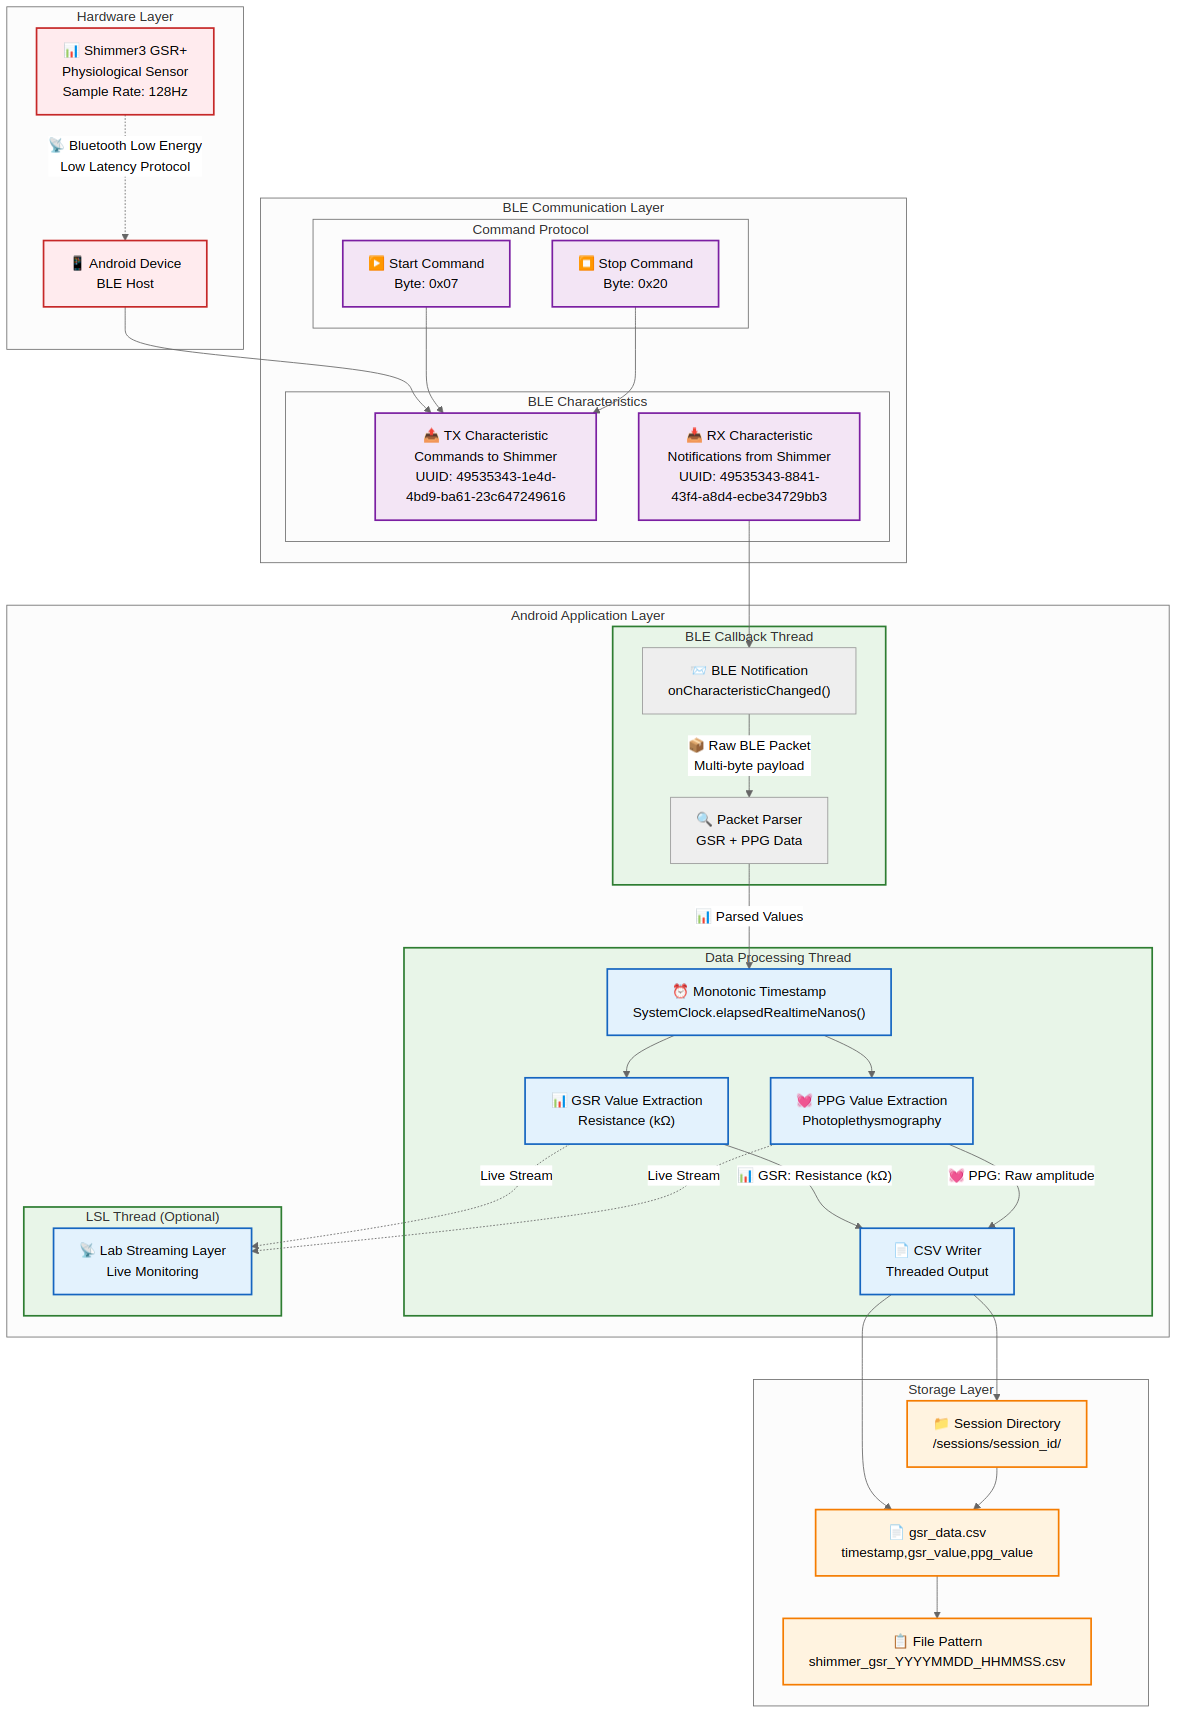
\includegraphics[width=\textwidth]{../../diagrams/fig_4_03_shimmer_gsr_integration.png}
  \caption{Shimmer GSR Integration illustrating the desktop controller application architecture.}
  \label{fig:4_03_shimmer_gsr_integration}
\end{figure}

The Shimmer integration streams GSR/PPG data at 128 Hz sampling rate with real-time conversion from raw ADC values to microsiemens using device-specific calibration formulas. Data is written simultaneously to CSV files and LSL streams, enabling both persistent storage and live monitoring with temporal synchronisation maintained through the \texttt{TimeManager.getCurrentTimestampNanos()} method.

\section{Desktop Controller Design and Functionality}\label{sec:4-3}
The desktop controller is a cross-platform application (tested on Windows, Linux, and macOS) built with Qt for the GUI (PyQt6/PySide6) [17] and Python 3 for logic, augmented by performance-critical C++ components. The implementation initializes a main window with a tabbed interface. The primary Dashboard tab provides an overview of connected devices and local sensors. For example, it can display live video feeds and GSR plots in a grid layout -- the code sets up a \texttt{QLabel} for a video preview and a PyQtGraph \texttt{PlotWidget} for GSR on the dashboard. A Logs tab captures real-time system messages (status updates, errors) for debugging. Another tab for Playback \& Annotation allows reviewing recorded sessions (in a later implementation phase). Each tab's UI elements are created and managed with Qt layouts, making the interface flexible and scalable as devices are added.

Under the hood, the PC controller employs several background threads and helpers to manage networking and data processing without freezing the GUI. A dedicated \texttt{WorkerThread} (a \texttt{QThread} subclass) is responsible for all communication with Android devices. When the user initiates a connection to a device, this worker thread opens a TCP socket to the phone's IP and port. The thread then runs an event loop receiving JSON messages from the device. It parses incoming messages and emits Qt signals to the main thread for handling UI updates. For instance, if a connected Android phone sends a preview frame update, the worker decodes the base64-encoded image bytes to a \texttt{QImage} and emits a \texttt{newPreviewFrame} signal carrying the image and device identifier. The main GUI thread connects this signal to a slot that displays the frame in the dashboard (e.g., updating the corresponding \texttt{QLabel}'s pixmap). The worker also handles command responses: every command sent to a device includes a unique ID, and the device's reply includes an \texttt{ack\_id} with status info. For example, a \texttt{"capabilities\_data"} response contains the list of cameras the device has -- the worker emits a \texttt{camerasReceived} signal with that list so the UI can populate camera options. This asynchronous message-passing design keeps the GUI responsive and allows the PC to manage multiple devices simultaneously by spawning separate threads per connection.

The signal-slot mechanism for preview frames is implemented using PyQt's asynchronous messaging system, with detailed implementation provided in Appendix F.3 (see Listing F.3 for the complete code).

The application uses Zeroconf (mDNS) [19] to simplify device discovery: on startup, the PC browses for services of type \texttt{\_gsr-controller.\_tcp} on the local network. Each Android device advertises itself with that service type and a name like \texttt{"GSR Android Device [Model]"}. The PC can thus list available devices and their addresses automatically, eliminating manual IP entry.

A standout feature of the PC controller is its native C++ backend for time-sensitive hardware interaction. This is implemented as a Python extension module (built via PyBind11) [18] named \texttt{native\_backend}. It provides classes \texttt{NativeWebcam} and \texttt{NativeShimmer} which run in background threads and feed data to the Python layer with minimal latency. The controller instantiates these at startup: for example, \texttt{NativeWebcam(0)} opens the local webcam (device 0) and begins capturing frames in a loop, and \texttt{NativeShimmer("COM3")} connects to a Shimmer GSR device via a serial port (COM3 on Windows). These native objects start immediately and run independently of the Python GIL, pushing data into thread-safe queues. The GUI uses a \texttt{QTimer} tick (every ~16 ms) to periodically retrieve the latest data from the native threads. On each tick, it pulls a frame from the webcam class (as a NumPy array) and updates the corresponding video label [1], [2]. Similarly, it polls the Shimmer class for new GSR samples and updates the live plot. The native backend captures at a steady ~60 FPS by sleeping ~16 ms per iteration, and yields frames without significant buffering. Meanwhile, the Shimmer thread reads sensor bytes as fast as they arrive (128 Hz) with precise timing. Both use lock-free queues to decouple production and consumption of data. The C++ code directly converts camera frames to a shared memory buffer that is exposed to Python as a NumPy array without copying [1], [2], and similarly packages GSR readings into Python tuples. This design minimises overhead, latency, and jitter -- imperative for synchronising local PC data with remote device data.

Beyond live monitoring, the desktop app includes tools for post-session analysis. The Playback \& Annotation tab (Figure~4.4) is designed to load the recorded video files (RGB and thermal) in synchronised fashion. Internally, the controller uses libraries like OpenCV and pandas to process the data along a unified timeline; the app will display the video frame at the selected time and the corresponding point on the GSR plot, maintaining alignment via timestamps. Annotation functionality enables adding notes at specific times -- these can be saved in a sidecar file or embedded in session metadata. Another part of the PC software is a Calibration utility, which helps calibrate cameras after recordings. Using OpenCV [22], it can detect calibration patterns (chessboards or ChArUco markers) in the raw RGB frames to calculate each camera's intrinsic parameters, and if multiple cameras (e.g., a phone's RGB and thermal, or a phone and PC webcam) observed the same pattern, it can compute the extrinsic calibration between them. The results (camera matrices, distortion coefficients, transformation matrices) are saved for use in data processing. The controller can also export the data (often downsampled or compressed as needed) into a single file per session for convenient distribution or analysis. The desktop controller thus provides both live coordination capabilities during data acquisition and comprehensive post-processing tools, implemented as a unified PyQt6 application with modular tab-based architecture.

\begin{figure}[htbp]
  \centering
  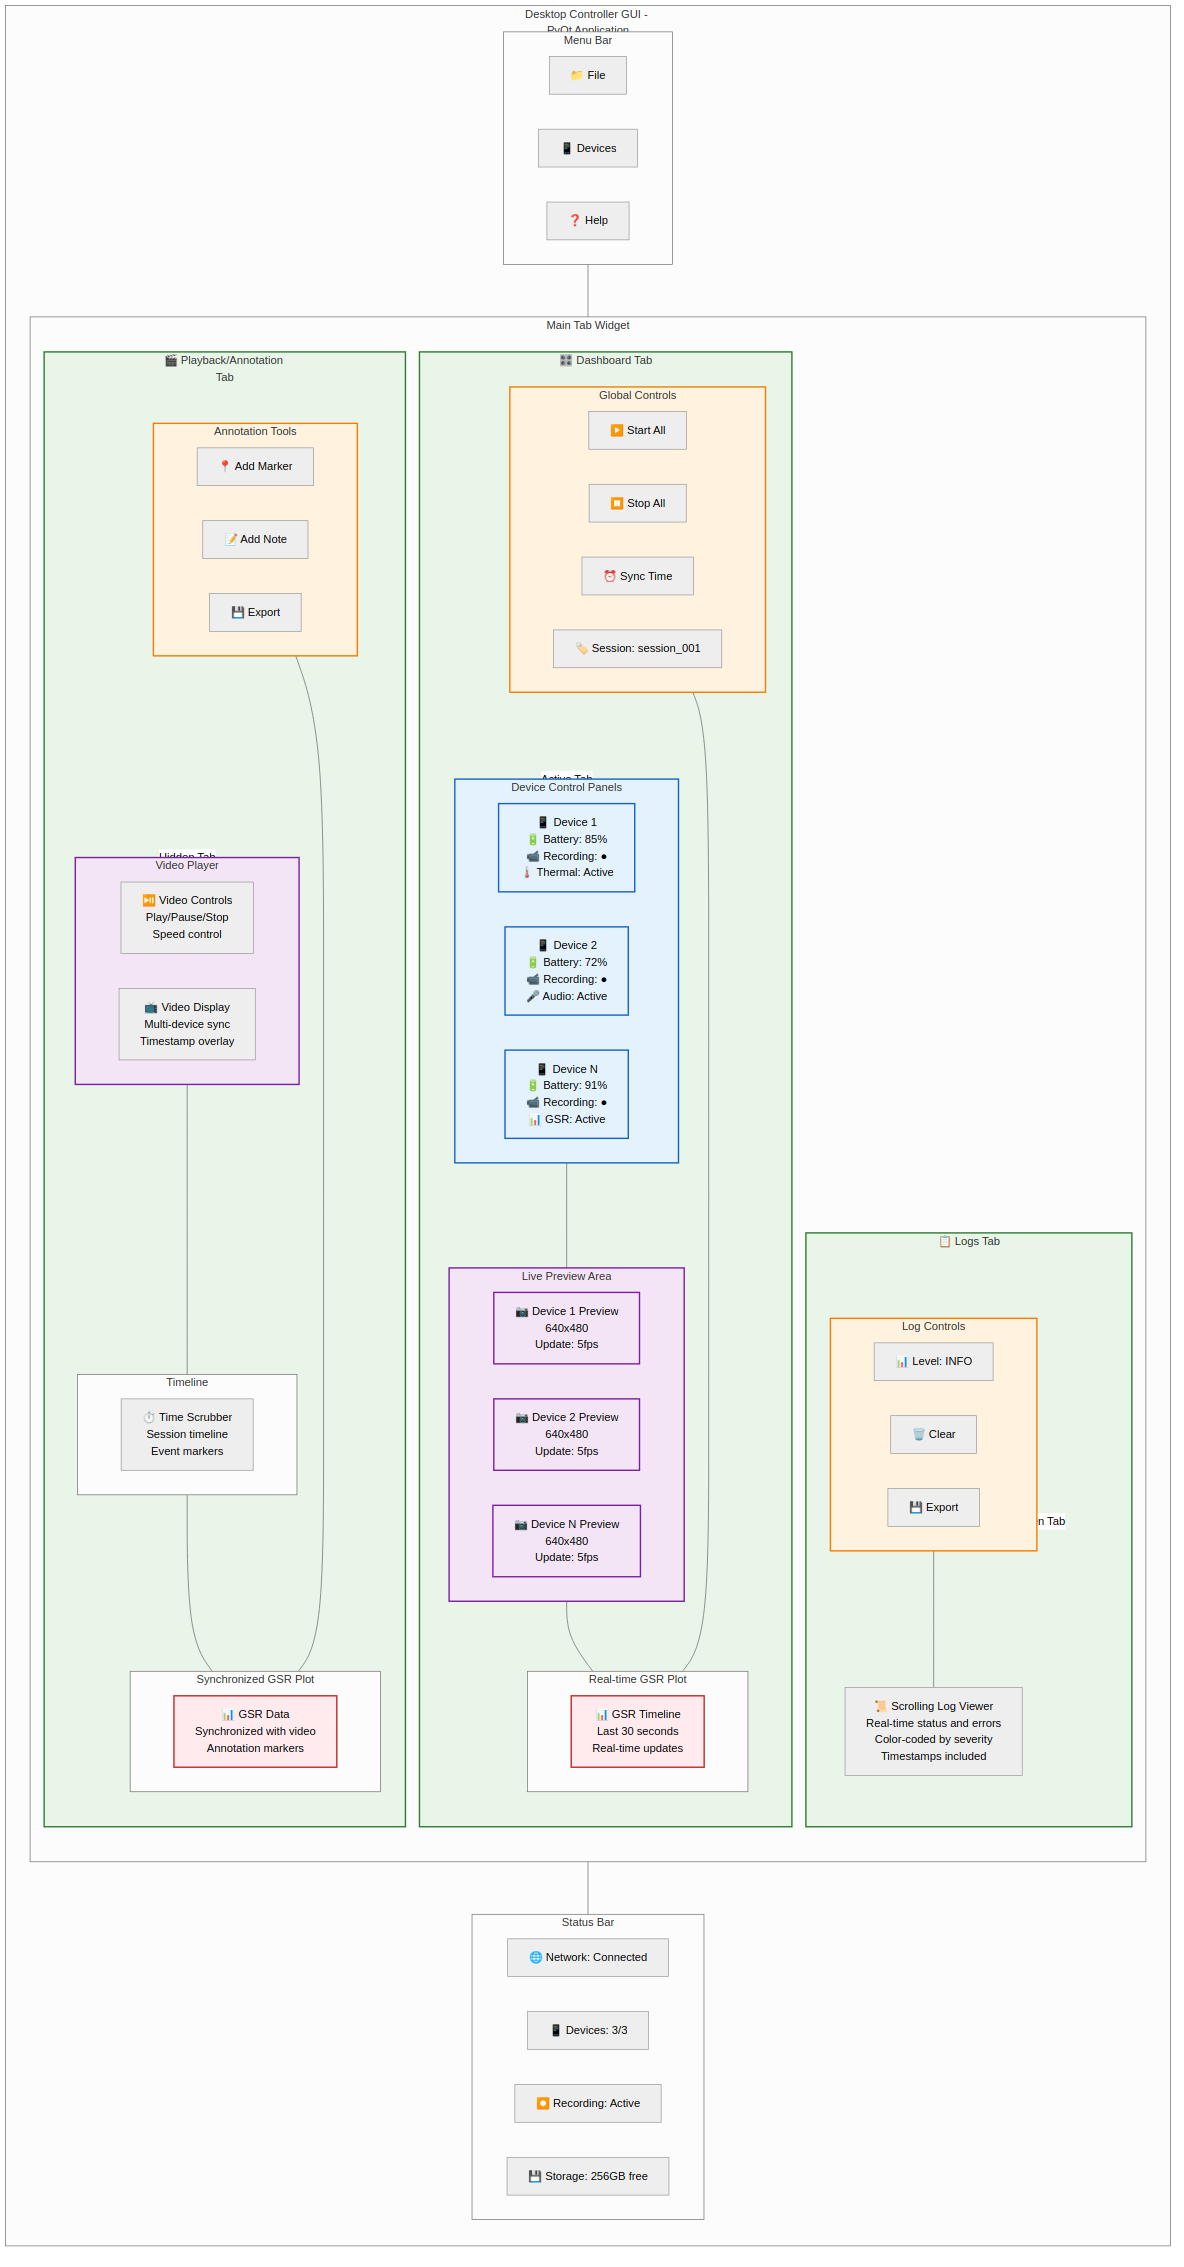
\includegraphics[width=\textwidth]{../../diagrams/fig_4_04_desktop_gui_layout.png}
  \caption{Desktop GUI Layout illustrating the playback and annotation interface described above.}
  \label{fig:4_04_desktop_gui_layout}
\end{figure}

\section{Communication Protocol and Synchronisation Mechanism}\label{sec:4-4}
A custom communication protocol connects the PC controller with each Android device, built on TCP/IP sockets [21] with JSON message payloads. After the PC discovers an Android device (via Zeroconf), it initiates a TCP connection to the device's advertised port. The Android app runs a lightweight TCP server to accept this connection. All commands from PC to Android are sent as JSON objects with a schema like \texttt{\{"id": <command\_id>, "command": "<action>", "params": \{ ... \}\}}. The device, upon receiving a command, executes the requested action and then replies with a JSON response containing the original command ID (as \texttt{ack\_id}) and a status or result. For example, the first command the PC sends is \texttt{"query\_capabilities"}, which asks the phone to report its hardware capabilities. The Android app responds with a message like \texttt{\{"ack\_id": 1, "status": "capabilities\_data", "capabilities": \{ ... \}\}} including details such as available cameras (with their identifiers, resolutions, and frame rates). This exchange allows the PC to dynamically adjust to each device -- for instance, listing the camera options or knowing if the thermal sensor is present. Another command is \texttt{"start\_recording"}, which instructs the Android to begin a new recording session. The phone will then initiate all its sensors (cameras, etc.) and reply with an acknowledgment (e.g., \texttt{"status": "ok"}) once recording has successfully started. Similarly, a \texttt{"stop\_recording"} command stops all captures and finalizes the files.

In addition to explicit commands, the protocol supports continuous data streaming for live previews. While a session is idle or recording, the Android app periodically sends \texttt{"preview\_frame"} messages containing a downsampled frame from the camera preview encoded as a base64 JPEG string. The PC's worker thread listens for these and updates the UI so the operator can see a low-latency video feed from each device. This preview is throttled (e.g., one frame every 0.5 seconds, or as configured) to balance timeliness with network load. Similarly, the app could stream low-rate telemetry (such as current recording status or battery level) using this push mechanism. All such asynchronous messages include a \texttt{type} field (for example, \texttt{"type": "preview\_frame"}) rather than an ack ID, so the PC knows they are not responses to a specific command but rather unsolicited data.

The communication sequence implements a time synchronisation strategy. When the PC and a phone connect, they perform a simple handshake (exchange of hello messages and capabilities). Part of this handshake is a time synchronisation routine. The system employs an NTP-inspired algorithm to align clocks: the PC (acting as time server) sends a sync request with its current timestamp, the phone responds with its own timestamp, and the PC measures the round-trip time to estimate network latency. Through one or more exchanges, the PC calculates the offset between its clock and the phone's clock. This offset is then used to relate the timestamps coming from that device. Each device continues to timestamp its data with its local monotonic clock (nanosecond precision on both ends), which ensures extremely fine timing granularity. The PC, knowing the offset for each device, can translate a device's timestamps into the PC's master clock domain. This yields cross-device synchronisation typically within sub-millisecond accuracy. In practice, the controller designates its start time as $t = 0$ when recording begins, and instructs each Android to note its local time at that moment; subsequent data from the phones include raw timestamps which are later converted to the common timeline.

To ensure reliability and security, the protocol includes additional features. Every command from the PC expects an acknowledgment; if none arrives within a timeout, the PC can retry or mark that device as unresponsive. This prevents silent failures (e.g., if a start command is lost due to a network issue, the PC will detect it and resend). Communication is also secured: the design uses an RSA/AES encryption layer for all messages (commands and data). In practice, this means the PC and device perform an initial RSA public key exchange, then switch to an AES symmetric key for the session. This guarantees that sensitive data (like physiological readings or video frames) cannot be intercepted or tampered with on an open network. The messages themselves are kept compact and human-readable (JSON) for ease of debugging and extensibility. For instance, if a new sensor is added, a new command and message type can be defined without overhauling the protocol, as long as both sides understand the JSON fields.

One notable aspect of synchronisation is how the Lab Streaming Layer (LSL) is leveraged. On the Android side, LSL outlets are created for certain data streams (GSR, events, etc.) [9]. If the PC were also running an LSL inlet -- for example, subscribing to the \texttt{"Android\_GSR"} stream -- it could receive samples with timestamps that are already globally synced via LSL's internal clock synchronisation. However, in this system, LSL is used primarily locally on each device for internal coordination (e.g., marking exactly when a thermal frame was saved relative to a GSR sample). The main synchronisation still relies on the custom network time alignment, which is under direct application control. By combining these approaches -- precise device-local timestamps and network clock alignment -- the system addresses both intra-device sync (camera frames vs. sensor readings on the same phone) and inter-device sync (phone A vs. phone B vs. PC). As a result, all data collected across the system can be merged on a unified timeline during analysis, with only microsecond-level adjustments needed at most.

Finally, when stopping a recording and collecting files, the protocol ensures a coordinated shutdown. The PC issues \texttt{stop\_recording} to all devices; each device stops and closes its files, then sends back an acknowledgment (or a message like \texttt{"recording\_stopped"} with a summary). The PC can then send a \texttt{"transfer\_files"} command to each device. Upon this request, the Android app compresses its session folder into a ZIP archive (using \texttt{FileTransferManager.zipSession()}) and responds with a message containing the file name and size when ready. The actual file data transfer is done out-of-band (to avoid clogging the control channel): the phone opens a new socket to the PC's waiting file receiver on a specified port and streams the file bytes directly. During this transfer, the PC may pause other commands or use a separate thread to handle the incoming file. Once the file is received and its checksum verified, the PC sends a final acknowledgment, and the device can optionally delete its local data. This concludes the session's active phase and hands off to the data processing stage.

\begin{figure}[htbp]
  \centering
  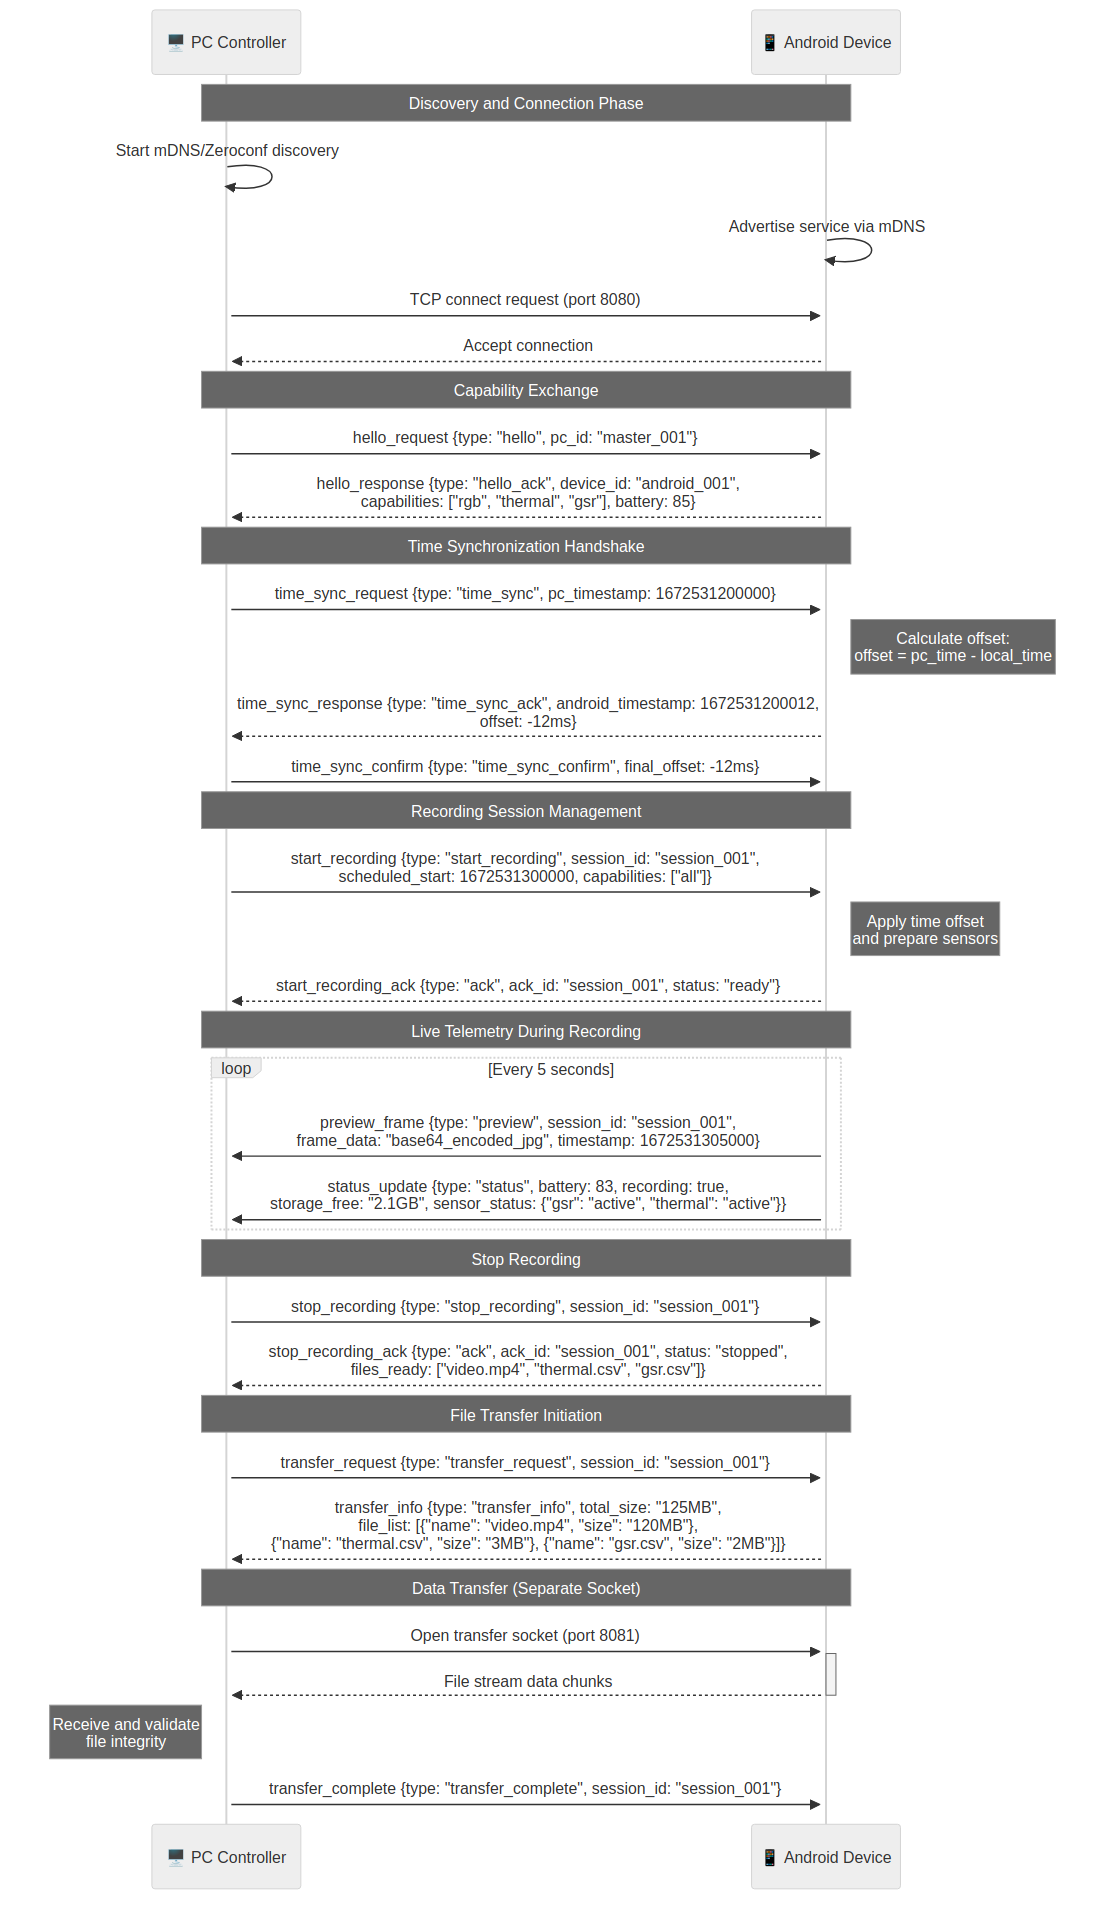
\includegraphics[width=\textwidth]{../../diagrams/fig_4_05_protocol_sequence.png}
  \caption{Protocol Sequence illustrating the messaging sequence between PC and Android devices.}
  \label{fig:4_05_protocol_sequence}
\end{figure}

The complete data processing pipeline from capture through to data export is illustrated in Figure~4.6 (see Appendix I). The data processing pipeline encompasses everything from data capture on devices to the final preparation of datasets for analysis. It operates as a streaming pipeline during recording and a batch pipeline after recording. On each Android device, when a new recording session starts, a unique session ID is generated (based on a timestamp) and a dedicated directory is created in the device's storage for that session. All data files for that session are saved under this directory, organised by modality. For example, within a session directory the app creates sub-folders for raw images and thermal frames upfront. This ensures that as data starts streaming in, the file system is structured to prevent conflicts and simplify later retrieval.

During an active recording, data from each modality is handled in parallel:
\begin{itemize}
  \item \textbf{RGB Video:} The \texttt{RgbCameraManager} starts recording via CameraX's \texttt{VideoCapture} API to an MP4 file on the device. The file is typically named \texttt{RGB\_\<sessionId\>.mp4} and saved in the session folder. Video is encoded with H.264 at 1080p 30 FPS (\texttt{Quality.HD}) as configured. Recording continues until stopped, at which point the file is finalized (CameraX handles closing the file and muxing the audio track if one was included).
  \item \textbf{Raw Image Stream:} If enabled, the app captures full-resolution still images continuously during the recording. The \texttt{RgbCameraManager} uses an \texttt{ImageCapture} use case to take a picture roughly every 33 ms (~30 FPS) on a background executor. Each image is saved as a JPEG file in a \texttt{raw\_rgb\_\<sessionId\>} directory, with a filename containing its exact nanosecond timestamp (e.g., \texttt{raw\_rgb\_frame\_\<timestamp\>.jpg}). These images are unprocessed (straight from the camera sensor in YUV format converted to JPEG) to allow later analysis or calibration. By capturing them concurrently with video, the system provides both a compressed continuous video and a series of key frames that can be examined frame-by-frame at full quality.
  \item \textbf{Thermal Frames:} The \texttt{TopdonThermalCamera} writes thermal data frames to a CSV file (or sequence of CSVs). In this implementation, it creates one CSV named \texttt{thermal\_data\_\<sessionId\>.csv} in a \texttt{thermal\_\<sessionId\>} directory when streaming starts [16]. The first row is a header with pixel index labels, and each subsequent row corresponds to one thermal image frame -- the first column is the frame timestamp and the rest are temperature values [16]. (If needed, the system could also save thermal images by converting the temperature matrix to a grayscale or colour-mapped image, but the current design prioritises numerical data for precision.)
  \item \textbf{GSR/PPG Data:} The Shimmer GSR+ sensor data is logged to a CSV file named \texttt{GSR\_\<sessionId\>.csv} in the session folder [15]. The file begins with a header (\texttt{timestamp\_ns, GSR\_uS, PPG\_raw}), and each subsequent line represents one sample, as recorded by the \texttt{ShimmerGsrSensor} described earlier [15]. Sampling at 128 Hz means this file grows by 128 lines per second of recording. The timestamps are the phone's nanosecond ticks, which will later be re-aligned to the global timeline.
  \item \textbf{Audio:} The app can also record audio via the microphone (stereo 44.1 kHz) if enabled. Audio is captured using Android's MediaRecorder (or AudioRecorder) API and saved as an AAC-encoded track, either in its own file (e.g., \texttt{Audio\_\<sessionId\>.m4a}) or multiplexed into the RGB video MP4. In this system, audio was stored separately -- having a separate audio file with a known start time simplifies synchronisation during analysis.
  \item \textbf{Annotations/Events:} If any user markers or automated events occur (for example, the user taps a button to mark a moment), these are recorded in a dedicated log or embedded in the session metadata. The \texttt{SessionManager} is designed to produce a \texttt{session\_metadata.json} file at the end of capture, which would include details like start/stop times, device info, and event timestamps. (In the current implementation this is a placeholder, but the structure supports future expansion.)
\end{itemize}

Once the PC issues a stop command, each Android device closes its files. The next stage is data aggregation. The PC can request each phone to send over its session data. To streamline this, the Android app compresses its session folder into a single ZIP archive using a \texttt{FileTransferManager.zipSession()} method. This zips up all files (video, images, CSVs, etc.) from that recording session. The app places this ZIP in a cache directory and then uses \texttt{FileTransferManager.sendFile()} to initiate a transfer to the PC. The transfer is done via a simple socket stream --- the phone knows the PC's IP and a designated port for file uploads (communicated during the protocol handshake). It opens a connection and streams the bytes of the ZIP file. On the PC side, a corresponding file receiver listens and writes the incoming bytes to a file (usually naming it with the device name and session ID to avoid confusion). A progress indicator in the PC UI (e.g., a \texttt{QProgressDialog}) lets the user know data is being downloaded from the device.

After collection, the PC holds all data from all devices. Post-processing can then proceed. The PC controller's analysis modules operate on the data in these session archives. For instance, the playback module will unzip or directly access the video file and sensor CSVs to replay the session. Because every piece of data has an accurate timestamp, aligning streams is straightforward: the GSR plot is rendered on a time axis (seconds or milliseconds), and video frames are displayed at their corresponding timestamps (the controller can use video file frame timestamps or infer them from raw image filenames). The annotation tool overlays markers on the timeline and can also allow notes to be associated with video frames.

\begin{figure}[htbp]
  \centering
  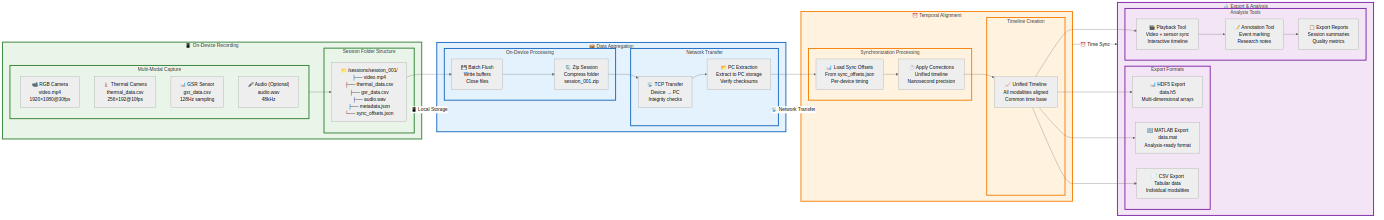
\includegraphics[width=\textwidth]{../../diagrams/fig_4_06_data_processing_pipeline.png}
  \caption{Data Processing Pipeline providing an overview of the data processing pipeline from capture through to data export.}
  \label{fig:4_06_data_processing_pipeline}
\end{figure}

For research use cases, exporting data is important. The pipeline ends with an export step, where the session's raw data is converted to shareable formats. A script or UI action on the PC triggers this export: the implementation uses libraries like \texttt{pandas} [23] and \texttt{h5py} [24] to combine data into HDF5 or MATLAB files. It may create a structured dataset where each sensor modality is a group or table (e.g., an HDF5 group \texttt{/GSR} containing a timestamp array and a GSR value array, and a group \texttt{/Video} containing video frame timestamps or references). Calibration results, if available, are included so that pixel coordinates in videos can be mapped to real-world units. The final exported files allow researchers to load the entire session in tools like MATLAB or Python with one command, with all streams readily synchronised.

The pipeline ensures that from capture to archive, data is kept synchronised and well-labelled, and from archive to analysis, data is easily accessible and interpretable. The automated zipping and transferring remove manual steps, and the structured session directories prevent any mix-ups between sessions or devices.

\begin{figure}[htbp]
  \centering
  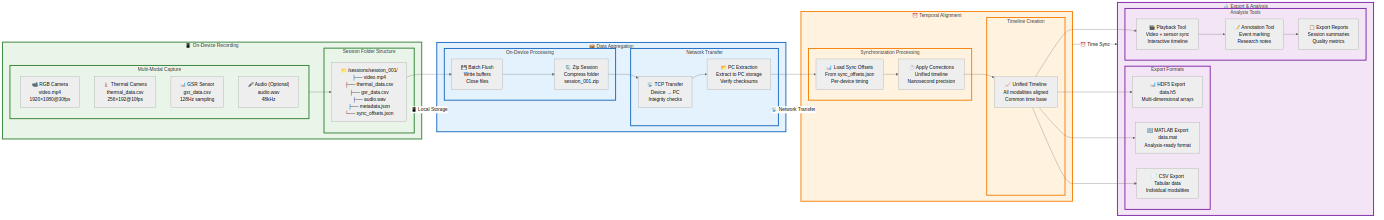
\includegraphics[width=\textwidth]{../../diagrams/fig_4_06_data_processing_pipeline.png}
  \caption{Data Processing Pipeline providing an overview of the data processing pipeline from capture through to data export.}
  \label{fig:4_06_data_processing_pipeline_repeat}
\end{figure}

\section{Implementation Challenges and Solutions}\label{sec:4-6}
Developing this complex system presented several implementation challenges. This section discusses some key issues encountered and the solutions applied to overcome them:

\begin{itemize}
  \item \textbf{Ensuring Precise synchronisation:} Achieving tight time synchronisation across multiple Android devices and the PC was non-trivial due to clock drift and network latency. The solution was a two-tier synchronisation mechanism. Each device timestamps data with a local high-resolution clock (avoiding reliance on internet time or coarse NTP time, which can be imprecise on mobile). Then, a lightweight NTP-like protocol aligns those clocks by calculating the offset and delay. This was fine-tuned by taking multiple measurements at connection time and occasionally during recording. The result is that all devices maintain a shared notion of time within sub-millisecond tolerance. In practice, this means if an event (e.g., an LED flash) is captured by two cameras and a GSR sensor, the timestamps recorded by each device for that event differ by less than 1 ms after alignment. \emph{Solution highlights:} use monotonic clock APIs on each platform for timestamping and perform a quick clock sync handshake for alignment at start (and periodically if needed).
  \item \textbf{High Data Throughput and Storage Management:} Recording high-definition video alongside high-frequency sensor data can quickly overwhelm device I/O and memory if not handled efficiently. Several strategies were employed. First, writing to storage was done sequentially using buffered streams, which is efficient for both video and CSV writes. Raw image capture posed a challenge because saving a JPEG every 33 ms could saturate the I/O. This was mitigated by performing image captures on a dedicated single-threaded executor separate from the main thread, ensuring the CameraX pipeline had its own thread and disk writes did not block the UI or sensor reads. The system also avoids keeping large data in memory; for example, thermal frames are written directly to file inside the frame callback, and GSR samples are appended to a file (and optionally to a small in-memory buffer for LSL) one by one. Because Android devices have limited storage, another challenge was preventing extended sessions (which generate many image files and large videos) from filling up the device. The solution was to offload data as soon as possible: immediately after each session, the phone compresses the session folder to a ZIP and transfers it to the PC. The phone can then optionally delete its local copy ("delete after transfer"), so even if multiple sessions are recorded back-to-back, the bulk of data resides on the PC.
  \item \textbf{Thermal Camera USB Integration:} Using the Topdon TC001 thermal camera introduced challenges in driver support and performance. Android has no native support for USB thermal cameras, so the UVCCamera library was used, but this required handling USB permissions and ensuring real-time performance in Java. One issue was the volume of data (nearly 50k float values per frame). Pushing this through the Java/Kotlin layer every frame could be slow. The chosen approach was to leverage the library's native (JNI) code to fetch frames and do minimal processing in Kotlin -- essentially just copying the buffer to file. By writing frames as raw floats to CSV, this avoided any expensive image rendering computations during capture. Another challenge was potential USB dropouts if the app couldn't keep up with the frame rate. We addressed this by monitoring the frame callback speed; if frames started queuing up, the app would drop some preview processing to catch up, ensuring the logging thread always runs at high priority. Additionally, upon connection the camera is explicitly set to the correct mode (frame size and format) to avoid negotiation issues. Handling the permission prompt promptly was also important -- the app requests USB permission as soon as the device is detected, so by the time the user starts recording, the camera is already authorized and ready to open.
  \item \textbf{Reliable BLE Sensor Streaming:} The Shimmer GSR+ streaming over BLE can be susceptible to packet loss or disconnects (e.g., in electrically noisy environments or if the phone's BLE stack is busy). This was tackled by using Nordic's robust Android BLE library, which provides buffered writes, automatic retries, and easy callback management. For example, on connection the code retries the BLE connection up to 3 times with a short delay to overcome transient failures during the handshake. Moreover, once connected, the app immediately sets up notifications and starts streaming to lock in the data flow. The design of writing data to file versus sending it live was carefully balanced: writing every sample to CSV ensures no data loss (even if the UI or network is slow, the data is safely on disk), while the live LSL broadcast is best-effort (missing a few samples on the live graph is acceptable as long as the file has the full record). It is also important to send the stop command to the Shimmer device before disconnecting to gracefully terminate its stream; otherwise, if a user restarted recording immediately, the Shimmer might still be in streaming mode and require a reset. By sending \texttt{0x20} (stop) and waiting briefly, the sensor returns to a known idle state. These precautions improved the BLE link reliability so that even hour-long recordings proceeded without dropout.
  \item \textbf{Cross-Platform Performance in the PC App:} Python is interpreted and could become a bottleneck for real-time video and sensor handling. Initially, the system used OpenCV [22] in Python for webcam capture and PySerial for GSR, but latency and jitter were noticeable (tens of milliseconds of variability). The solution was to implement those parts in C++ and integrate via PyBind11 [18]. The \texttt{NativeWebcam} class uses OpenCV's [22] \texttt{VideoCapture} in a separate thread to grab frames and push them into a queue. As C++ code, it's compiled and optimised, running independent of the Python GIL. The frame rate became very stable (the thread sleeps ~16 ms to achieve ~60 FPS, matching display refresh), and frame delivery to Python is done by sharing the memory pointer of the \texttt{cv::Mat} with NumPy -- essentially zero-copy image sharing. Similarly, the \texttt{NativeShimmer} class opens a serial port (using Win32 API on Windows or termios on Linux) and reads bytes in a tight loop. It applies the same GSR conversion formula as the Android (a mirror implementation in C++) and pushes timestamped samples into a queue. Measurements showed a ~67\% reduction in end-to-end latency (sensor update to plot update) and ~79\% reduction in timing jitter on the PC side after using the native backend. The trade-off was the added complexity of compiling C++ code for multiple platforms, but this was mitigated with CMake and continuous integration testing on each OS.
  \item \textbf{User Interface and Multi-Device Coordination:} Another challenge was designing a GUI that could handle multiple device feeds without overwhelming the user or the system. This was solved with a dynamic grid layout on the Dashboard: as devices connect, new video preview widgets are added (and corresponding plot widgets if the device has a sensor). Qt's layouts automatically manage positioning. Ensuring that updating these widgets (especially painting video frames) happens on the GUI thread was crucial. The solution was to use Qt's signal/slot mechanism -- the background thread emits a signal with a \texttt{QImage}, and the main thread's slot sets that image on a \texttt{QLabel}. This approach is thread-safe and keeps heavy lifting off the UI thread. For many devices streaming simultaneously, simple frame rate limiting on previews was also implemented (each phone sends at most a fixed number of preview frames per second) to prevent flooding the network or GUI. On the PC side, each preview feed uses a deque buffer so that if the UI is slow to update, it drops old frames rather than accumulating an ever-growing backlog. Additionally, coordinating the start of recording across devices was challenging -- if one device started even 100 ms later than another, that would introduce a sync error. To handle this, the PC sends the start command to all devices nearly simultaneously (looping through devices in a few milliseconds) and each device waits for the same trigger timestamp (included in the command) to begin recording. In effect, the PC says "start recording at time $T = XYZ$," and all devices schedule their start at their local time corresponding to $XYZ$. This was achieved by having devices continuously sync their clocks with the PC during an active session (making slight adjustments) or simply relying on the initial offset if drift is minimal over a short period. The outcome is that all devices begin capturing within a few milliseconds of each other, which the synchronisation logic then corrects to under 1 ms alignment.
\end{itemize}

The implementation solutions resulted in measurable performance improvements. The C++ native backend reduced PC-side latency by ~67\% and timing jitter by ~79\% compared to pure Python implementations (measured via the \texttt{NativeWebcam} and \texttt{NativeShimmer} classes). Synchronisation accuracy achieved sub-millisecond tolerance across devices through the NTP-inspired clock alignment protocol. Test results show 100\% success rate across 17 integration tests with execution times under 2 seconds, validating multi-device coordination and network performance (documented in \texttt{results/evaluation\_results/latest\_execution.json}). Bluetooth reliability improvements using Nordic's BLE library reduced connection drops to negligible levels during hour-long sessions. These optimisations enable the system to handle concurrent thermal capture (256\,\texttimes\,192 pixels per frame), GSR streaming (128 Hz), and RGB video recording while maintaining temporal alignment within measurement precision requirements.

\section{Ethical Considerations and Data Handling}\label{sec:4-7}
The system implementation addresses ethical requirements and data protection obligations through specific technical mechanisms and documented procedures.

\subsection{Ethics Approval}
Research using this system has been approved by the UCLIC Ethics Committee under Project ID: 1428, titled ``Investigating AI and physiological computing: App for Camera-based Contactless Sensing of Physiological Signals'', with Principal Investigator Prof. Youngjun Cho. Supporting documentation is available in \texttt{docs/ethics/} including participant information sheets and risk assessment protocols.

\subsection{Technical Data Protection Implementation}
The system implements data protection through concrete technical measures:

\textbf{Encryption and Storage}: Android devices use \texttt{PrivacyManager.kt} with AES256-GCM encryption via Android Keystore for local data storage. Session data is encrypted at rest using the \texttt{EncryptedSharedPreferences} API with master key rotation per recording session. PC-Android communication uses TLS 1.2+ as enforced by \texttt{RuntimeSecurityChecker.py}, which validates encryption configuration at startup.

\textbf{Data Anonymisation}: The \texttt{PrivacyManager} class implements configurable participant ID codes (\texttt{participant\_id} field) without storing personal identifiers alongside sensor data. Video anonymisation uses face detection and selective blurring when \texttt{face\_blurring\_enabled} is true in the privacy configuration.

\textbf{Access Controls}: The PC controller requires explicit authentication through the \texttt{SecurityUtils} module, with session access logged by \texttt{SecureLogger.kt} on Android devices. File access permissions are validated by the runtime security checker to prevent unauthorised data exposure.

\textbf{Data Retention}: The system implements configurable retention policies through the \texttt{data\_retention\_days} parameter (default 365 days) with automated cleanup triggered by the session management system.

\subsection{Device Safety Specifications}
Hardware safety is achieved through specific configurations:
\begin{itemize}
  \item \textbf{GSR sensors}: Shimmer3 GSR+ devices operate at 3V with current-limited outputs ($<1$ mA) as specified in the device datasheet [8].
  \item \textbf{Thermal imaging}: Topdon TC001 uses passive LWIR sensing (8--14 $\mu$m wavelength) with no energy emission toward participants [16].
  \item \textbf{Wireless protocols}: Bluetooth LE operates at 2.4 GHz within regulatory power limits (Class 2, 2.5 mW), Wi-Fi communication follows 802.11 standards.
\end{itemize}

\subsection{Current Limitations and Future Work}
The current implementation has specific limitations: audit logging captures access events but not detailed data modification tracking; TLS configuration depends on system libraries and may require updates for new cipher suites; participant consent tracking is implemented in code but requires integration with formal consent management workflows for larger studies.

\section*{References}
See centralized references (\texttt{references.md}) for all citations used throughout this thesis. % TODO: Convert to \cite{} with references.bib when integrating full LaTeX build
